\subsection*{You Only Look Once}

Der Algorithmus \textit{You Only Look Once} (YOLO) ist ein weiterer Objekterkennungsalgorithmus und betrachtet statt separaten Bildregionen das komplette Bild. Er benutzt nur ein neuronales Netz, um Bounding Boxen und Wahrscheinlichkeiten für bestimmte Klassen gleichzeitig vorherzusagen. Daher der Name \glqq You Only Look Once\grqq{}.

Hierzu wird ein $S \times S$ Gitter über das Bild gelegt. Für jedes Feld im Gitter werden durch ein einziges \textit{CNN} $B$ Bounding Boxen vorhergesagt, als auch zur Zelle dazugehörige Klassenwahrscheinlichkeiten. Für jede Bouding Box wird nun der \textit{confidence score} berechnet. Basierend auf diesem \textit{confidence score} wird ein Regressionsproblem zur richtigen Lokalisation gelöst. Aus der Menge der resultierenden Bounding Boxen werden schließlich mit Hilfe eines festgelegten Schwellwertes für den \textit{confidence score} die Boxen mit lokalisierten Objekten bestimmt (siehe Abbildung \ref{yolo_model}) \cite{JosephRedmon.2016}.

\begin{figure}[ht]
	\begin{center}
		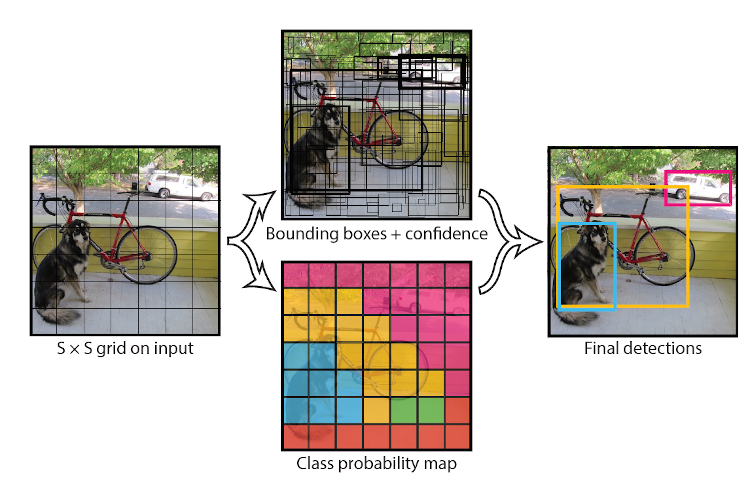
\includegraphics[width=15cm]{Bilder/yolo_model.png} 
		\caption[Vereinfachte Darstellung des YOLO Algorithmus]{Vereinfachte Darstellung des YOLO Algorithmus \cite{JosephRedmon.2016}}
		\label{yolo_model}
	\end{center}
\end{figure}

\newpage

Die vorhergesagten Werte werden in einem $S \times S \times (B * 5 + C)$ Tensor kodiert, wobei $S$ und $B$ wie zuvor beschrieben durch das Gitter und die Bounding Boxen festgelegt sind und $C$ die Anzahl der Klassen beschreibt. Abbildung \ref{yolo_architecture} zeigt den Aufbau des CNN von \textit{YOLO} für die Detektion. Es besteht aus 24 \textit{Convolutional Layern} zur Feature Extraktion gefolgt von zwei \textit{Fully-Connected} Layern, um die Klassenwahrscheinlichkeiten und Bounding Box Koordinaten zu bestimmen. Für die Genauigkeit bei der Detektion wird die Auflösung des Eingangsbildes verdoppelt \cite{JosephRedmon.2016}. 

In dem Netzwerk in Abbildung \ref{yolo_architecture} wird ein Bild mit einer Auflösung von $224 \times 224$ Pixeln verwendet und die vorhergesagten Werte im $7 \times 7 \times 30$ Tensor ausgegeben.

\begin{figure}[ht]
	\begin{center}
		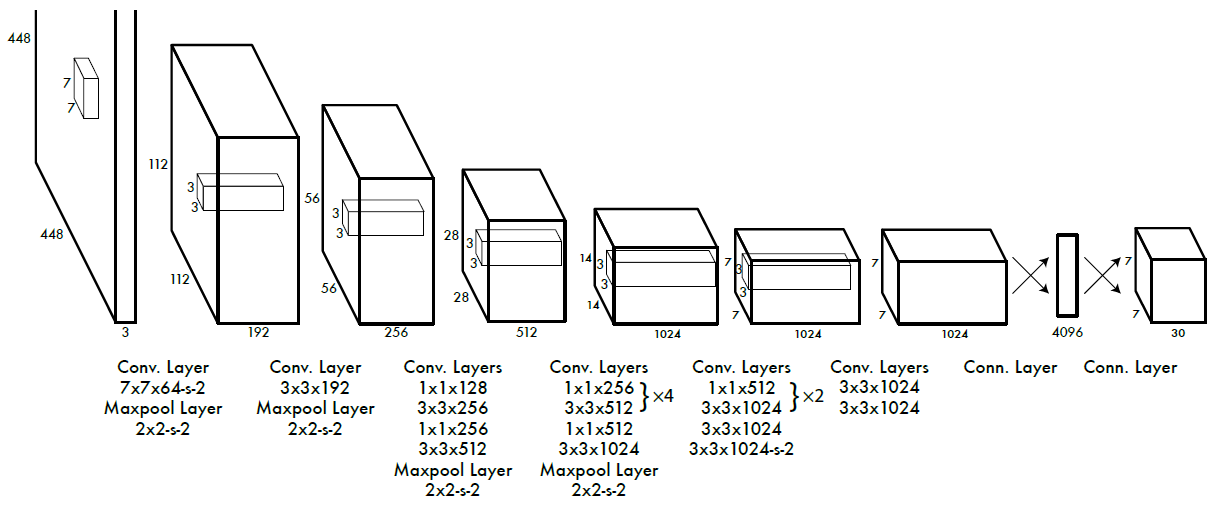
\includegraphics[width=15cm]{Bilder/yolo_architecture.png} 
		\caption[YOLO Architektur]{YOLO Architektur \cite{JosephRedmon.2016}}
		\label{yolo_architecture}
	\end{center}
\end{figure}

Die mittlerweile dritte und aktuelle Version von \textit{YOLO} weist einige Verbesserungen auf, gerade im Bezug auf die Erkennung von sehr kleinen Objekten wie zum Beispiel einzelnen Vögeln in einem Schwarm. Das in \textit{YOLOv3} verwendete \textit{CNN} umfasst insgesamt 53 \textit{Convolutional Layer} und entstand aus mehreren Optimierungsschritten des in Abbildung \ref{yolo_architecture} dargestellten \textit{CNN} \cite{JosephRedmon.2018}. 





